
\vspace*{1cm}
\supplementarysection

\begin{longtblr}[
  theme=ntabs,
  caption = {Model information}, % Table caption
  label = {table:model_info} % Label for cross-referencing
  % note{a} = {Continued from previous page}, % Note for continued header
  % note{b} = {Continued on next page}, % Note for continued footer
]{
  colspec = {X[l] X[6,l] X[l] X[l] X[l]}, % Define column specification
  column{1}={colsep=15pt},
  rowhead=1,
  row{odd} = {tablegrey}, % Shading for odd rows
  cells = {font = \fontsize{8pt}{8pt}\selectfont},
  row{1} = {tableheadgrey, font=\fontsize{8pt}{8pt}\selectfont\bfseries} % First row is bold
}

Model & Formula & Family & N & Groups \\

\addlinespace
\SetCell[c=5]{c, white}\textbf{Individual Repertoires} \\

% Individual Repertoires
rep\_m\_1 & repertoire\_size $\sim$ 1 + immigrant + s(sampling\_effort) + year + (1 | father) & cratio & 301 & 242 \\
rep\_m\_1.1 & repertoire\_size $\sim$ 1 + dispersal\_distance + s(sampling\_effort) + year + (1 | father) & cratio & 133 & 105 \\
rep\_m\_1.2 & repertoire\_size $\sim$ 1 + age + s(sampling\_effort) + year + (1 | father) & cratio & 256 & 205 \\
repnov\_m\_1 & average\_frequency $\sim$ 1 + immigrant + s(sampling\_effort) + year + (1 | father) & lognormal & 300 & 242 \\
repnov\_m\_1.1 & average\_frequency $\sim$ 1 + dispersal\_distance + s(sampling\_effort) + year + (1 | father) & lognormal & 133 & 105 \\
repnov\_m\_1.2 & average\_frequency $\sim$ 1 + age + s(sampling\_effort) + year + (1 | father) & lognormal & 256 & 205 \\

% Cultural Similarity
\SetCell[c=5]{c, white}\textbf{Cultural Similarity} \\
disp\_m\_1 & mean\_dist1 $\sim$ 0 + natal\_distance + nest\_distance + year\_born\_diff + year + (1 | mm(father, father2)) & Gaussian & 8745 & 105 \\
imm\_m\_1 & mean\_dist1 $\sim$ 0 + resident\_status + year\_born\_diff + nest\_distance + year + (1 | mm(father, father2)) & Gaussian & 11029 & 205 \\
age\_m\_1 & mean\_dist1 $\sim$ 0 + natal\_distance + nest\_distance + year\_born\_diff + year + (1 | mm(father, father2)) & Gaussian & 8745 & 105 \\

% Cultural Novelty and Diversity
\SetCell[c=5]{c, white}\textbf{Cultural Novelty and Diversity} \\
nov\_m\_1 & uniqueness $\sim$ 0 + prop\_immigrant + mean\_dispersal\_distance + prop\_same\_birds + mean\_age + s(n\_current\_songs) + year + gp(x, y, by = year) & lognormal & 791 & GP \\
div\_m\_1 & diversity $\sim$ 0 + prop\_immigrant + mean\_dispersal\_distance + prop\_same\_birds + mean\_age + s(n\_current\_songs) + year + gp(x, y, by = year) & lognormal & 791 & GP \\
nov\_m\_2 & uniqueness $\sim$ 0 + diversity + s(n\_current\_songs) + year + gp(x, y, by = year) & lognormal & 791 & GP \\
nov\_m\_2.1 & uniqueness $\sim$ 0 + diversity + year + gp(x, y, by = year) & lognormal & 791 & GP \\
div\_m\_2 & n\_unique\_current\_songs $\sim$ 0 + prop\_immigrant + mean\_dispersal\_distance + prop\_same\_birds + mean\_age + s(recorded) + year + gp(x, y, by = year) & Gaussian & 791 & GP \\
div\_m\_2.1 & n\_unique\_current\_songs $\sim$ 0 + prop\_immigrant + mean\_dispersal\_distance + prop\_same\_birds + mean\_age + s(n\_current\_songs) + year + gp(x, y, by = year) & Gaussian & 791 & GP \\

% Cultural Turnover
\SetCell[c=5]{c, white}\textbf{Cultural Turnover} \\
turn\_m\_1 & prop\_shared $\sim$ 0 + prop\_same\_birds + year + gp(x, y, by = year, k = 25, c = 5/4) & hurdle lognormal & 544 & GP \\
turn\_m\_2 & prop\_shared $\sim$ 0 + prop\_immigrant + mean\_dispersal\_distance + mean\_age + prop\_same\_birds + year + gp(x, y, by = year, k = 25, c = 5/4) & hurdle lognormal & 544 & GP \\
\end{longtblr}
\begin{longtblr}[
  theme=ntabs,
  caption = {Model estimates}, % Table caption
  label = {table:model_estimates}, % Label for cross-referencing
  note{a} = {Estimates are Medians and 95\% Credible Intervals}, % Note for continued header
]{
  colspec = {X[l] X[3,l] X[3,l] X[1.5,l] X[1.5,l]}, % Define column specification
  column{1}={colsep=15pt},
  rowhead=1,
  % rowsep=0pt,
  row{odd} = {tablegrey}, % Shading for odd rows
  cells = {font = \fontsize{8pt}{8pt}\selectfont},
  row{1} = {tableheadgrey, font=\fontsize{8pt}{8pt}\selectfont\bfseries} % First row is bold
}

Model & Hypothesis & Estimate\TblrNote{a} & Evid. Ratio & Post. Prob \\

\addlinespace
\SetCell[c=5]{c, white}\textbf{Individual Repertoires} \\

% Individual Repertoires
rep\_m\_1 & immigrant $>$ 0 & 0.239 [-0.098, 0.593] & 6.963 & 0.874 \\
rep\_m\_1.1 & dispersal distance $<$ 0 & -0.201 [-0.443, 0.045] & 10.111 & 0.910 \\
rep\_m\_1.2 & age $>$ 0 & 0.064 [-0.108, 0.241] & 2.701 & 0.730 \\
repnov\_m\_1 & non-immigrant $<$ 0 & -0.049 [-0.2, 0.1] & 2.401 & 0.706 \\
repnov\_m\_1.1 & dispersal distance $>$ 0 & 0.203 [0.088, 0.316] & 741.857 & 0.999 \\
repnov\_m\_1.2 & age $>$ 0 & -0.017 [-0.093, 0.058] & 0.540 & 0.351 \\

% Cultural Similarity
\SetCell[c=5]{c, white}\textbf{Cultural Similarity} \\
disp\_m\_1 & natal distance $>$ 0 & 0.001 [0, 0.002] & 22.529 & 0.958 \\
disp\_m\_1 & nest distance $>$ 0 & -0.005 [-0.006, -0.004] & Inf & 1 \\
imm\_m\_1 & both resident-both immigrant $<$ 0 & 0.002 [-0.005, 0.01] & 0.438 & 0.304 \\
imm\_m\_1 & both resident-one immigrant $<$ 0 & 0.002 [-0.002, 0.006] & 0.331 & 0.248 \\
age\_m\_1 & age difference 0-1 $>$ 0 & 0.002 [0, 0.003] & 12.289 & 0.925 \\
age\_m\_1 & age difference 0-2 $>$ 0 & 0.004 [0.002, 0.006] & Inf & 1 \\
age\_m\_1 & age difference 0-3 $>$ 0 & 0.006 [0.003, 0.008] & 1999 & 1 \\
age\_m\_1 & age difference 0-4+ $>$ 0 & 0.01 [0.006, 0.013] & Inf & 1 \\

% Cultural Novelty and Diversity
\SetCell[c=5]{c, white}\textbf{Cultural Novelty and Diversity} \\
nov\_m\_1 & mean dispersal distance $<$ 0 & -0.018 [-0.023, -0.012] & Inf & 1 \\
nov\_m\_1 & proportion immigrant $<$ 0 & 0.001 [-0.005, 0.006] & 0.752 & 0.429 \\
nov\_m\_1 & mean age $<$ 0 & 0.012 [0.005, 0.019] & 399 & 0.998 \\
nov\_m\_1 & individual turnover $<$ 0 & 0.001 [-0.005, 0.008] & 1.733 & 0.634 \\
div\_m\_1 & mean dispersal distance $<$ 0 & -0.005 [-0.01, 0] & 26.65 & 0.964 \\
div\_m\_1 & proportion immigrant $<$ 0 & 0.002 [-0.004, 0.007] & 0.442 & 0.306 \\
div\_m\_1 & mean age $<$ 0 & 0.021 [0.014, 0.027] & Inf & 1 \\
div\_m\_1 & individual turnover $<$ 0 & -0.002 [-0.008, 0.005] & 0.446 & 0.309 \\
nov\_m\_2 & diversity $>$ 0 & 0.713 [0.629, 0.795] & Inf & 1 \\
nov\_m\_2.1 & diversity $>$ 0 & -0.099 [-0.216, 0.018] & 0.086 & 0.080 \\
div\_m\_2 & mean dispersal distance $<$ 0 & -0.658 [-0.999, -0.315] & 570.429 & 0.998 \\
div\_m\_2 & proportion immigrant $<$ 0 & 0.469 [0.1, 0.837] & 62.492 & 0.984 \\
div\_m\_2 & mean age $<$ 0 & 1.045 [0.576, 1.495] & Inf & 1 \\
div\_m\_2 & individual turnover $<$ 0 & 0.204 [-0.291, 0.683] & 3.077 & 0.755 \\
div\_m\_2.1 & mean dispersal distance $<$ 0 & 0.019 [-0.213, 0.249] & 0.824 & 0.452 \\
div\_m\_2.1 & proportion immigrant $<$ 0 & 0.072 [-0.168, 0.312] & 2.259 & 0.693 \\
div\_m\_2.1 & mean age $<$ 0 & 0.928 [0.599, 1.245] & Inf & 1 \\
div\_m\_2.1 & individual turnover $<$ 0 & -0.031 [-0.349, 0.279] & 0.726 & 0.421 \\

% Cultural Turnover
\SetCell[c=5]{c, white}\textbf{Cultural Turnover} \\
turn\_m\_1 & individual turnover $>$ 0 & 0.072 [0.054, 0.09] & Inf & 1 \\
turn\_m\_2 & mean dispersal distance $<$ 0 & -0.022 [-0.039, -0.006] & 79 & 0.988 \\
turn\_m\_2 & proportion immigrant $<$ 0 & -0.051 [-0.065, -0.037] & Inf & 1 \\
turn\_m\_2 & mean age $<$ 0 & -0.044 [-0.063, -0.026] & 3999 & 1 \\
turn\_m\_2 & individual turnover $<$ 0 & 0.047 [0.028, 0.066] & Inf & 1 \\
\end{longtblr}



\begin{figure}[tbp]
    \centering
    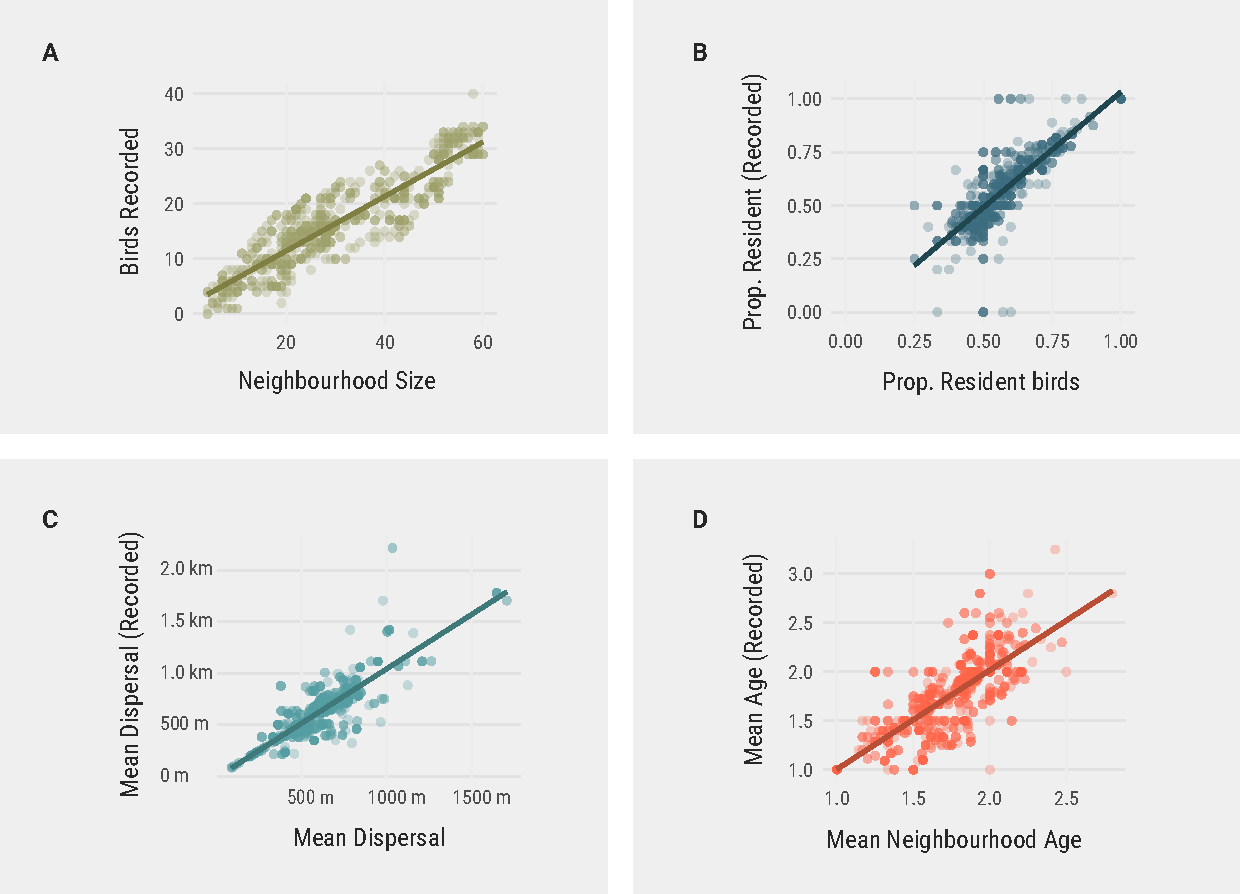
\includegraphics[width=\linewidth]{figures/chapter_4/supp_neighbourhood_sampling.pdf}
    \mycaption{Absence of bias in the sampling of neighbourhood properties}{
        Correlation between the actual neighbourhood properties and neighbourhood properties estimated from birds for which we have song recordings.
    (A) Neighbourhood size (number of individuals) and number of individuals with song recordings.
    (B) Proportion of resident birds from monitoring data and only those birds with song recordings.
    (C) Mean dispersal distance calculated from birds born in the study site and only those birds born in the study site with song recordings.
    (D) Mean age of birds in the study site and only those birds with song recordings.
    }
    \label{fig:supp_neighbourhood_sampling}
\end{figure}


\begin{figure}[tbp]
    \centering
    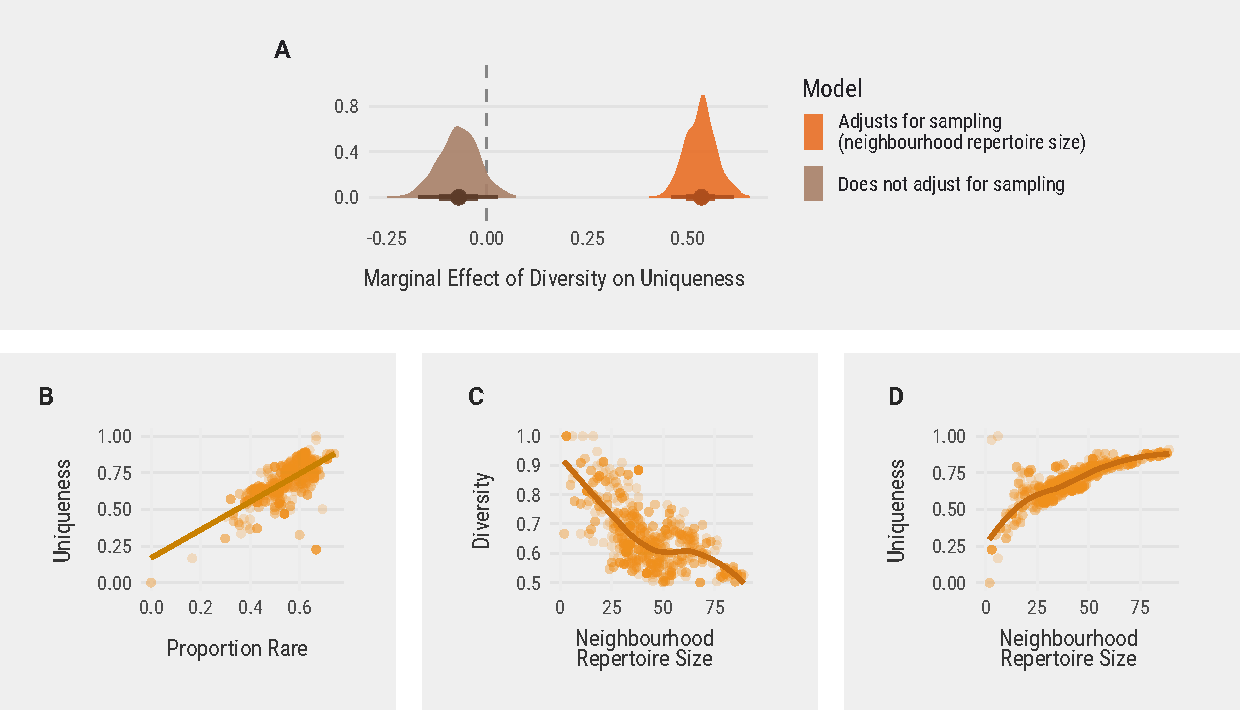
\includegraphics[width=\linewidth]{figures/chapter_4/supp_song_sampling.pdf}
    \mycaption{Relationships among outcome variables and sampling effects}{
        (A) Marginal effect of diversity---which describes the proportion of unique songs in a neighbourhood---on novelty, that is, how uncommon, on average, the songs of the birds in a neighbourhood are. These two ways of characterising cultural diversity are (as expected) anti-correlated in our study site due to the effect of sampling: more frequent songs are sampled more readily, causing larger sample sizes (neighbourhoods with more birds and therefore songs) to yield lower average estimates of diversity (C) and higher average estimates of novelty (D), in a nonlinear manner. Once this is adjusted for, diversity and novelty are positively correlated, as expected. (B) Our measure of cultural novelty (y-axis) has the advantages of being continuous and not using an arbitrary cutoff, but is nonetheless correlated with definitions traditionally used in the literature, such as “songs shared by fewer than 4 birds” \parencite{mcgregor1982b}}
    \label{fig:supp_song_sampling}
\end{figure}

\begin{figure}[tbp]
    \centering
    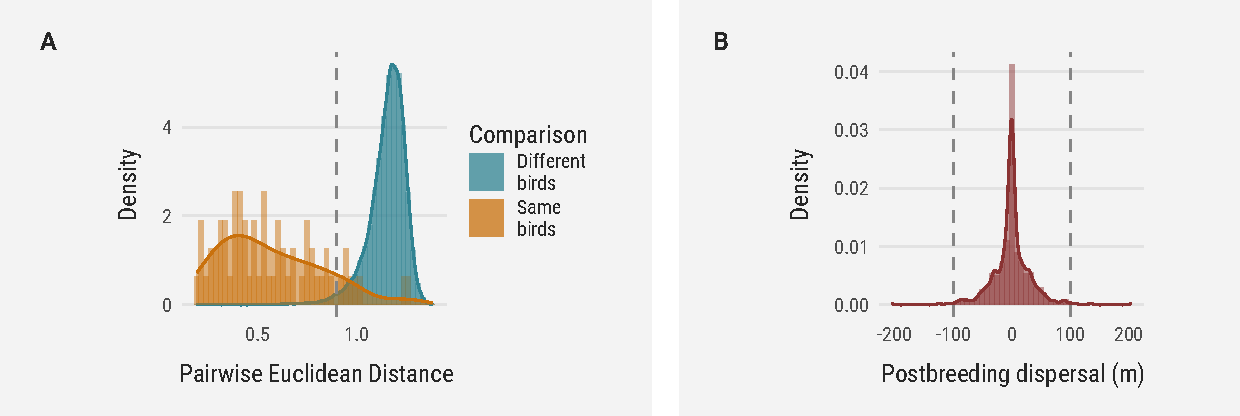
\includegraphics[width=\linewidth]{figures/chapter_4/supp_acoustic_distance_threshold.pdf}
    \mycaption{Thresholds used during the process of reidentifying individual birds based on their songs}{
        (A) Shows the distribution of the acoustic distances between the same song type sung by the same known bird in different years, in orange, and the minimum pairwise distance between different birds and years. The x-intercept of the vertical line = 0.9. (B) Shows the distribution of the change in distance from the natal nest box to the breeding site in different years for birds that bred more than once. Adult birds have high nest site fidelity, which we used as a further constraint when reidentifying them from their songs.}
    \label{fig:supp_acoustic_distance_threshold}
\end{figure}


\begin{figure}[tbp]
    \centering
    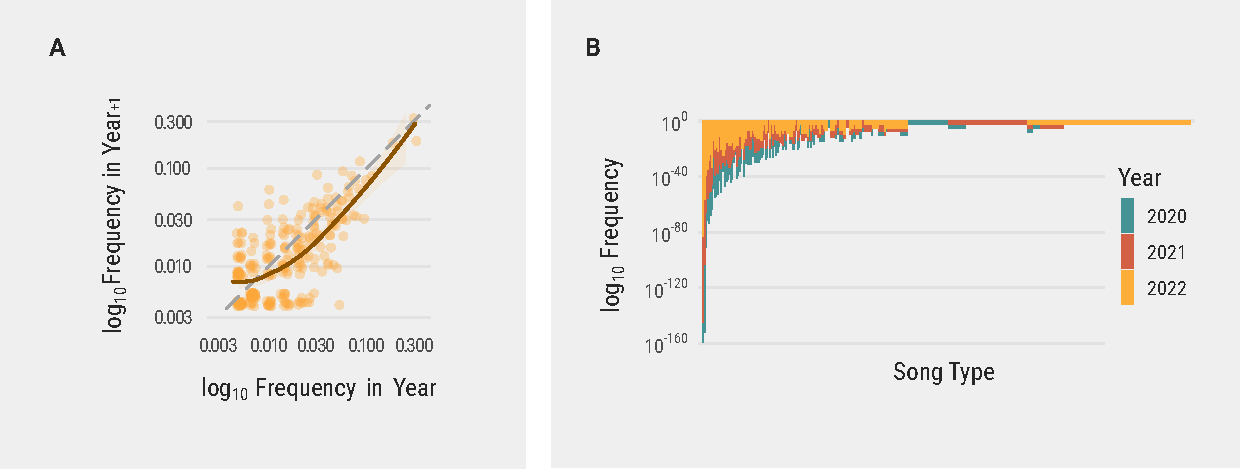
\includegraphics[width=\linewidth]{figures/chapter_4/supp_song_frequencies.pdf}
    \mycaption{
        Song frequencies and their relationship with abundance in the following year}{
        (A) The abundance of a song type in a given year predicts its abundance in the following year, with higher variance around rare songs. (B) Histogram showing the frequency of individual spong types in the study.
    }
    \label{fig:supp_song_frequencies}
\end{figure}


\begin{figure}[tbp]
    \centering
    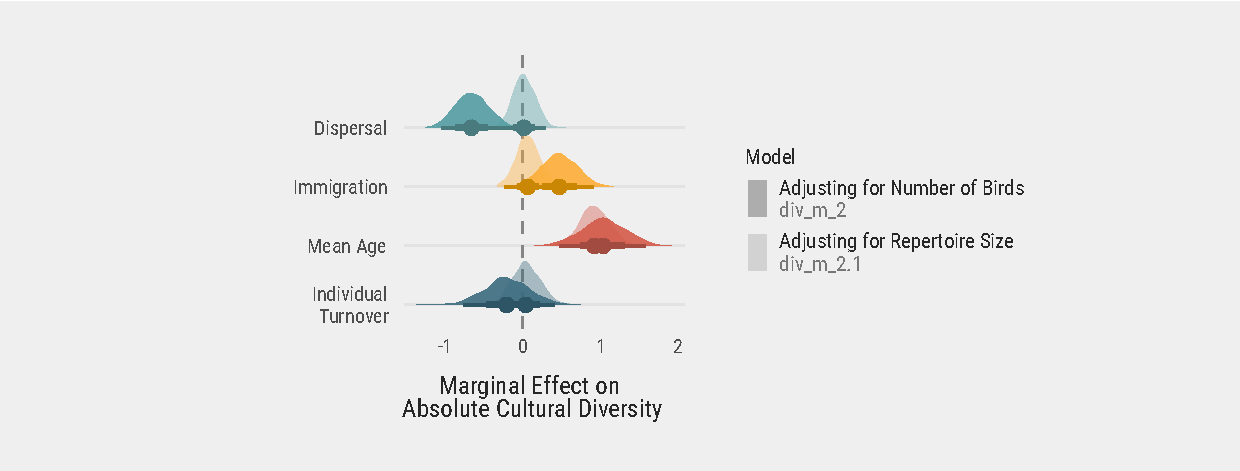
\includegraphics[width=\linewidth]{figures/chapter_4/supp_absolute_cultural_diversity.pdf}
    \mycaption{Marginal effects of demographic variables on absolute cultural diversity}{
        Marginal effects of our predictor variables on absolute cultural diversity (the number of different song types sampled in a neighbourhood), while adjusting for the effect of either number of individuals (higher opacity fill, corresponding to model \textit{div\_m\_2}) or number of song variants, including repeated variants (lower opacity fill, \textit{div\_m\_2.1}). 
    }
    \label{fig:supp_absolute_cultural_diversity}
\end{figure}



\begin{figure}[tbp]
    \centering
    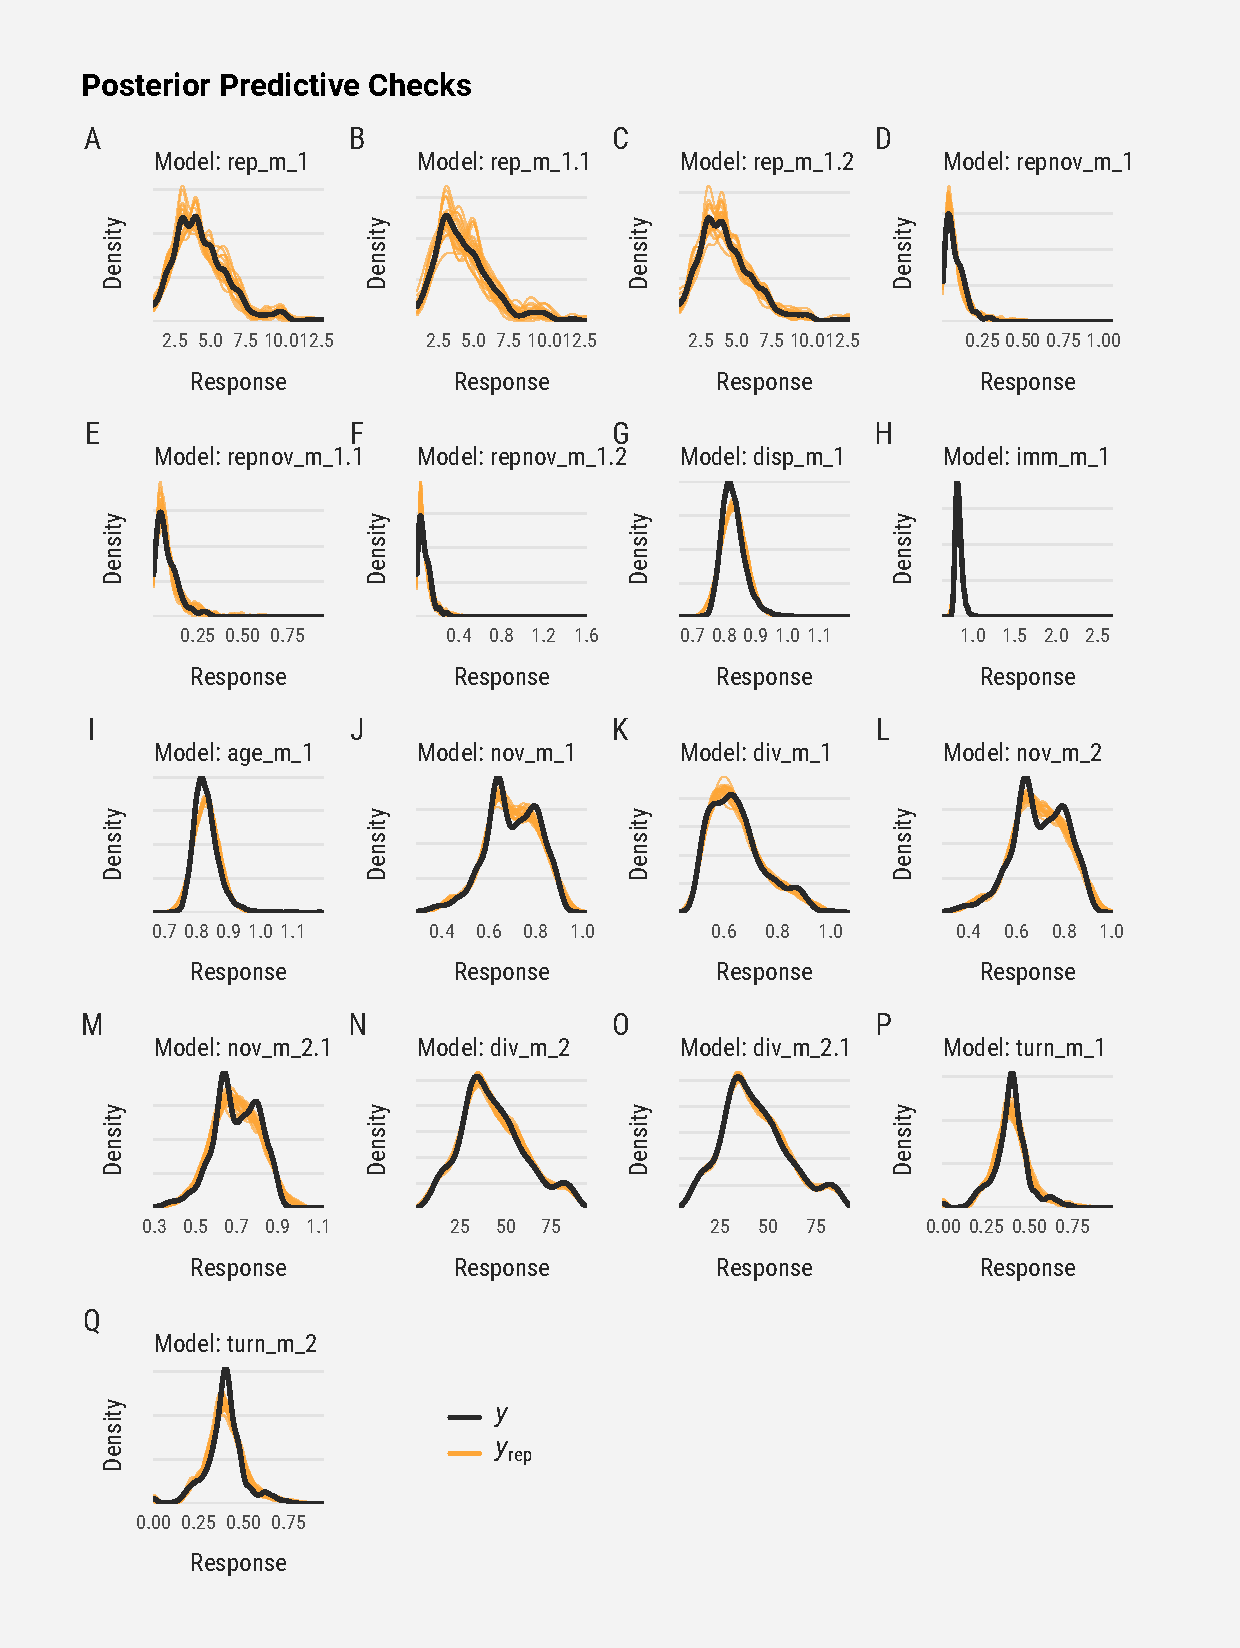
\includegraphics[width=\linewidth]{figures/chapter_4/supp_pp_checks.pdf}
    \mycaption{
        Posterior predictive checks for the main models in the study}{Comparing simulations from the posterior predictive distribution $y^{rep}$ (thin orange lines) with the outcome $y$ (black lines) using Kernel density estimates. The posterior predictive distribution is a distribution of possible outcomes of the model given the data and the model parameters, here used to check the fit of the model to the data.
    }
    \label{fig:supp_pp_checks}
\end{figure}

